\documentclass[12pt,a4paper]{article}

\usepackage{amsmath}
\usepackage{fontspec}
\usepackage{unicode-math}
\setmainfont{Times New Roman}
\setsansfont{Calibri}
\setmathfont{Cambria Math}
\usepackage{geometry}
\geometry{top=2.2cm,bottom=2.2cm,left=2.4cm,right=2.0cm}
\usepackage{graphicx}
\usepackage{xcolor}
\usepackage{array}
\usepackage{booktabs}
\usepackage{longtable}
\usepackage{float}
\usepackage{placeins}
\usepackage{enumitem}
\usepackage{fancyhdr}
\usepackage{tikz}
\usetikzlibrary{arrows.meta,calc,positioning}
\usepackage{hyperref}
\hypersetup{colorlinks=true,linkcolor=blue!55!black,urlcolor=blue!55!black}
\usepackage{titlesec}

\setlength{\parindent}{0pt}
\setlength{\parskip}{5pt}
\emergencystretch=3em
\renewcommand{\arraystretch}{1.18}
\renewcommand{\contentsname}{Mục lục}
\renewcommand{\figurename}{Hình}
\renewcommand{\tablename}{Bảng}

\definecolor{criticalbar}{RGB}{211,47,47}
\definecolor{normalbar}{RGB}{63,125,190}
\definecolor{weekend}{RGB}{235,235,235}

\pagestyle{fancy}
\fancyhf{}
\lhead{\small Quản trị dự án}
\rhead{\small Bach Minh Quang - 202490077}
\cfoot{\thepage}
\setlength{\headheight}{15pt}

\titleformat{\section}{\Large\bfseries\color{blue!55!black}}{\thesection.}{0.5em}{}
\titleformat{\subsection}{\large\bfseries\color{blue!45!black}}{\thesubsection}{0.5em}{}

\tikzset{
  event/.style={circle,draw=black,thick,minimum size=8mm,inner sep=1pt,
    font=\scriptsize,align=center},
  arc/.style={-{Latex[length=2mm]},thick,blue!65!black},
  criticalarc/.style={-{Latex[length=2mm]},very thick,criticalbar},
  dummyarc/.style={-{Latex[length=2mm]},dashed,gray!70!black},
  arclabel/.style={font=\scriptsize,fill=white,inner sep=1pt}
}

\newcommand{\ganttrowseven}[5]{%
  \node[anchor=east,font=\scriptsize] at (-0.25,-#1+0.18) {#2};%
  \pgfmathtruncatemacro{\gLast}{#4-1}%
  \foreach \gK in {0,...,\gLast}{%
    \pgfmathtruncatemacro{\gStart}{#3+\gK}%
    \fill[#5] (\gStart,-#1) rectangle ++(1,0.34);%
  }%
}

\newcommand{\ganttrowfive}[5]{%
  \node[anchor=east,font=\scriptsize] at (-0.25,-#1+0.18) {#2};%
  \pgfmathtruncatemacro{\gLast}{#4-1}%
  \foreach \gK in {0,...,\gLast}{%
    \pgfmathtruncatemacro{\gWork}{#3+\gK}%
    \pgfmathtruncatemacro{\gWeek}{int(\gWork/5)}%
    \pgfmathtruncatemacro{\gCal}{\gWork+2*\gWeek}%
    \fill[#5] (\gCal,-#1) rectangle ++(1,0.34);%
  }%
}

\newcommand{\ganttlegend}[1]{%
  \fill[criticalbar] (0,-#1) rectangle +(0.55,0.28);
  \node[anchor=west,font=\tiny] at (0.7,-#1+0.14) {Công việc găng};
  \fill[normalbar] (8.8,-#1) rectangle +(0.55,0.28);
  \node[anchor=west,font=\tiny] at (9.5,-#1+0.14) {Công việc không găng};
}

\begin{document}

\begin{titlepage}
\thispagestyle{empty}
\begin{center}
  {\large\bfseries ĐẠI HỌC BÁCH KHOA HÀ NỘI}\\[4pt]
  {\large\bfseries TRƯỜNG CÔNG NGHỆ THÔNG TIN VÀ TRUYỀN THÔNG}\\[1.5cm]
  \rule{\textwidth}{0.8pt}\\[0.55cm]
  {\Large\bfseries BÁO CÁO BÀI TẬP}\\[0.35cm]
  {\LARGE\bfseries QUẢN TRỊ DỰ ÁN}\\[0.55cm]
  \rule{\textwidth}{0.8pt}\\[1.5cm]
  
\begin{tikzpicture}
    \draw[blue!55!black,very thick] (0,0) circle (1.25cm);
    \draw[criticalbar,very thick] (-0.62,0.45) -- (0.18,0.45) -- (0.62,-0.35);
    \draw[normalbar,very thick] (-0.62,-0.25) -- (-0.05,-0.25) -- (0.62,0.35);
    \node[font=\small\bfseries] at (0,-1.65) {PERT - CPM - GANTT};
  \end{tikzpicture}\\[1.5cm]
  \begin{tabular}{rl}
    \textbf{Sinh viên:} & Bach Minh Quang\\
    \textbf{Mã sinh viên:} & 202490077\\
    \textbf{Học phần:} & Quản trị dự án\\
  \end{tabular}\\[2.0cm]
  {\large Hà Nội, tháng 09 năm 2026}
\end{center}
\end{titlepage}

\tableofcontents
\clearpage

\section*{Lời mở đầu}
\addcontentsline{toc}{section}{Lời mở đầu}

Báo cáo này trình bày lời giải cho năm bài tập PERT/CPM theo mẫu tham khảo
trong thư mục học phần. Mỗi bài gồm dữ liệu công việc, mạng PERT, thời điểm
sớm nhất và muộn nhất của các sự kiện, đường găng, dự trữ và biểu đồ Gantt theo
hai loại lịch: tuần làm việc 7 ngày và tuần làm việc 5 ngày.

Đề bài không quy định ngày bắt đầu cụ thể. Vì vậy, các biểu đồ Gantt dùng mốc
tương đối: ngày công việc thứ 0 là ngày khởi động dự án và trong biểu đồ 5 ngày,
mốc này được xem là thứ Hai. Khi nhập dữ liệu vào MS Project, chỉ cần thay ngày
bắt đầu hoặc chọn lịch \texttt{Standard} (thứ Hai đến thứ Sáu) và \texttt{7 Days};
quan hệ trước - sau và số ngày công việc không thay đổi.

\section{Cơ sở tính toán}

\subsection{Ký hiệu và công thức}

Với một cung công việc $i \rightarrow j$ có thời gian $d_{ij}$, ký hiệu:

\begin{itemize}[leftmargin=1.8em]
  \item $t_s(i)$: thời điểm sớm nhất của sự kiện $i$;
  \item $t_m(i)$: thời điểm muộn nhất của sự kiện $i$ mà không làm trễ dự án;
  \item $ES,EF$: thời điểm bắt đầu và kết thúc sớm của công việc;
  \item $LS,LF$: thời điểm bắt đầu và kết thúc muộn của công việc.
\end{itemize}

Tính tiến:
\[
  t_s(j)=\max_{i\rightarrow j}\{t_s(i)+d_{ij}\},\qquad
  ES_{ij}=t_s(i),\qquad EF_{ij}=t_s(i)+d_{ij}.
\]
Tính lùi từ sự kiện kết thúc có thời điểm bằng thời gian dự án:
\[
  t_m(i)=\min_{i\rightarrow j}\{t_m(j)-d_{ij}\},\qquad
  LS_{ij}=t_m(j)-d_{ij},\qquad LF_{ij}=t_m(j).
\]

Ba loại dự trữ được dùng trong báo cáo:
\[
\begin{aligned}
  TF_{ij}&=LF_{ij}-ES_{ij}-d_{ij},\\
  FF_{ij}&=t_s(j)-t_s(i)-d_{ij},\\
  IF_{ij}&=\max\{0,\ t_s(j)-t_m(i)-d_{ij}\}.
\end{aligned}
\]

Trong đó $TF$ là dự trữ toàn phần, $FF$ là dự trữ tự do và $IF$ là dự trữ
độc lập theo định nghĩa PERT. Công việc có $TF=0$ được gọi là công việc găng.
Để trả lời ý "có thể đồng thời kéo dài tất cả các công việc không găng",
báo cáo lấy mức kéo dài chung bằng giá trị nhỏ nhất của $TF$ trong tập các
công việc không găng. Mức này không làm thay đổi thời gian hoàn thành dự án.

\subsection{Quy ước biểu đồ}

Trong các sơ đồ PERT, số trong vòng tròn là số hiệu sự kiện; dòng dưới là
$t_s/t_m$. Cung màu đỏ là cung găng, cung màu xanh là cung không găng, còn
cung nét đứt là công việc giả có thời gian bằng 0, dùng để thể hiện quan hệ
trước - sau. Trong các biểu đồ Gantt, mỗi ô màu tương ứng một ngày công việc;
phần màu xám ở biểu đồ 5 ngày là thứ Bảy và Chủ nhật.

\clearpage
\section{Bài tập 1}

\subsection{Dữ liệu}

\begin{table}[H]\centering
\caption{Dữ liệu công việc của Bài tập 1}
\begin{tabular}{c c c}
\toprule
\textbf{Công việc} & \textbf{Trình tự} & \textbf{Thời gian (ngày)}\\
\midrule
A & Từ đầu & 2\\
B & Sau A & 1\\
C & Từ đầu & 1\\
D & Sau B, C & 1\\
G & Từ đầu & 3\\
H & Sau D, G & 3\\
F & Từ đầu & 2\\
I & Sau H, F & 2\\
\bottomrule
\end{tabular}
\end{table}

\subsection{Sơ đồ PERT và chỉ tiêu sự kiện}

\begin{figure}[H]\centering
\resizebox{0.96\linewidth}{!}{%
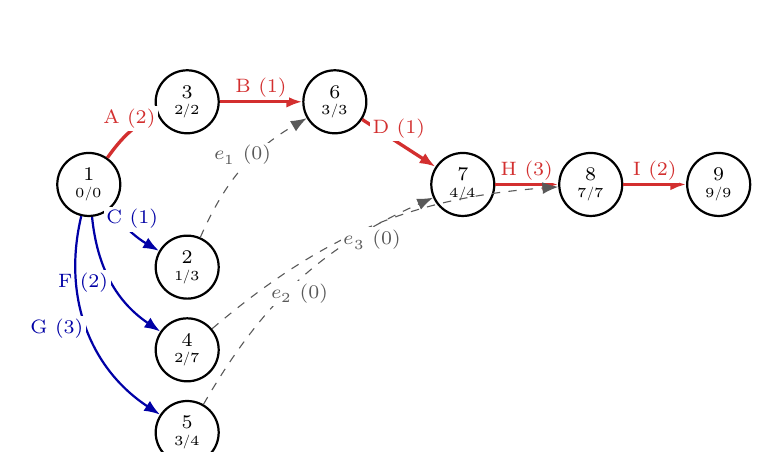
\begin{tikzpicture}[x=1.25cm,y=1.05cm]
  \node[event] (p1) at (0,1) {1\\[-2pt]\tiny $0/0$};
  \node[event] (p2) at (1,0) {2\\[-2pt]\tiny $1/3$};
  \node[event] (p3) at (1,2) {3\\[-2pt]\tiny $2/2$};
  \node[event] (p4) at (1,-1) {4\\[-2pt]\tiny $2/7$};
  \node[event] (p5) at (1,-2) {5\\[-2pt]\tiny $3/4$};
  \node[event] (p6) at (2.5,2) {6\\[-2pt]\tiny $3/3$};
  \node[event] (p7) at (3.8,1) {7\\[-2pt]\tiny $4/4$};
  \node[event] (p8) at (5.1,1) {8\\[-2pt]\tiny $7/7$};
  \node[event] (p9) at (6.4,1) {9\\[-2pt]\tiny $9/9$};
  \draw[criticalarc] (p1) to[bend left=15] node[arclabel,above] {A (2)} (p3);
  \draw[arc] (p1) to[bend right=10] node[arclabel,above] {C (1)} (p2);
  \draw[arc] (p1) to[bend right=25] node[arclabel,left] {F (2)} (p4);
  \draw[arc] (p1) to[bend right=35] node[arclabel,left] {G (3)} (p5);
  \draw[criticalarc] (p3) -- node[arclabel,above] {B (1)} (p6);
  \draw[dummyarc] (p2) to[bend left=18] node[arclabel,above] {$e_1$ (0)} (p6);
  \draw[criticalarc] (p6) -- node[arclabel,above] {D (1)} (p7);
  \draw[dummyarc] (p5) to[bend left=18] node[arclabel,below] {$e_2$ (0)} (p7);
  \draw[criticalarc] (p7) -- node[arclabel,above] {H (3)} (p8);
  \draw[dummyarc] (p4) to[bend left=18] node[arclabel,below] {$e_3$ (0)} (p8);
  \draw[criticalarc] (p8) -- node[arclabel,above] {I (2)} (p9);
\end{tikzpicture}}
\caption{Mạng PERT của Bài tập 1}
\end{figure}

\begin{table}[H]\centering
\caption{Thời điểm sớm và muộn của các sự kiện - Bài tập 1}
\begin{tabular}{c|rrrrrrrrr}
\toprule
Sự kiện & 1&2&3&4&5&6&7&8&9\\
\midrule
$t_s$ & 0&1&2&2&3&3&4&7&9\\
$t_m$ & 0&3&2&7&4&3&4&7&9\\
\bottomrule
\end{tabular}
\end{table}

\subsection{Tính dự trữ và đường găng}

\begin{longtable}{c|r|rr|rr|rrr}
\caption{Các chỉ tiêu thời gian của công việc - Bài tập 1}\\
\toprule
\textbf{CV}&\textbf{$d$}&\textbf{ES}&\textbf{EF}&\textbf{LS}&\textbf{LF}&\textbf{TF}&\textbf{FF}&\textbf{IF}\\
\midrule
\endfirsthead
\toprule
\textbf{CV}&\textbf{$d$}&\textbf{ES}&\textbf{EF}&\textbf{LS}&\textbf{LF}&\textbf{TF}&\textbf{FF}&\textbf{IF}\\
\midrule
\endhead
A&2&0&2&0&2&0&0&0\\
B&1&2&3&2&3&0&0&0\\
C&1&0&1&2&3&2&0&0\\
D&1&3&4&3&4&0&0&0\\
G&3&0&3&1&4&1&0&0\\
H&3&4&7&4&7&0&0&0\\
F&2&0&2&5&7&5&0&0\\
I&2&7&9&7&9&0&0&0\\
\bottomrule
\end{longtable}

Thời gian ngắn nhất của dự án là \textbf{9 ngày}. Đường găng là
\[
  \boxed{A-B-D-H-I}.
\]
Các công việc không găng là $C,G,F$, có dự trữ toàn phần lần lượt là
2, 1 và 5 ngày. Vì vậy, nếu kéo dài đồng thời tất cả các công việc không
găng, mức kéo dài chung lớn nhất là \textbf{1 ngày}. Theo công thức dự trữ
độc lập PERT, các công việc không găng của mạng này đều có $IF=0$.

\subsection{Biểu đồ Gantt}

\begin{figure}[H]\centering
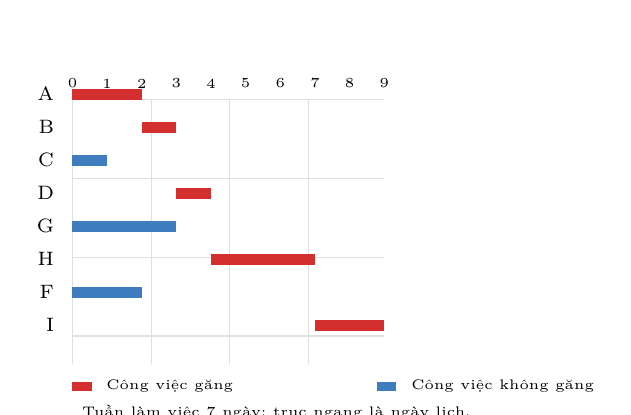
\begin{tikzpicture}[x=0.44cm,y=0.42cm]
  \draw[gray!25] (0,0) grid (9,-8);
  \foreach \x in {0,...,9} \node[font=\tiny,anchor=south] at (\x,0.06) {\x};
  \ganttrowseven{0}{A}{0}{2}{criticalbar}
  \ganttrowseven{1}{B}{2}{1}{criticalbar}
  \ganttrowseven{2}{C}{0}{1}{normalbar}
  \ganttrowseven{3}{D}{3}{1}{criticalbar}
  \ganttrowseven{4}{G}{0}{3}{normalbar}
  \ganttrowseven{5}{H}{4}{3}{criticalbar}
  \ganttrowseven{6}{F}{0}{2}{normalbar}
  \ganttrowseven{7}{I}{7}{2}{criticalbar}
  \ganttlegend{8.8}
  \node[font=\tiny,anchor=west] at (0,-9.45) {Tuần làm việc 7 ngày; trục ngang là ngày lịch.};
\end{tikzpicture}
\caption{Gantt Bài tập 1 - lịch 7 ngày}
\end{figure}

\begin{figure}[H]\centering
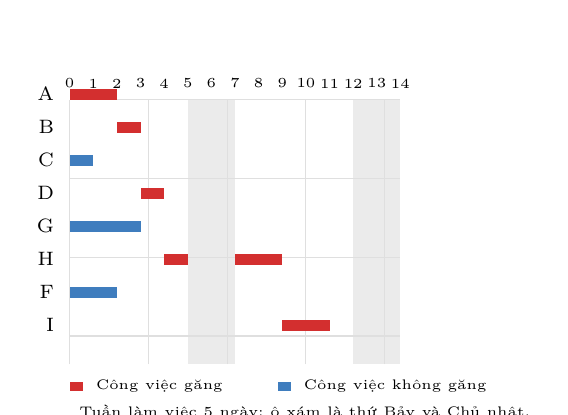
\begin{tikzpicture}[x=0.30cm,y=0.42cm]
  \foreach \w in {0,1} {\fill[weekend] ({7*\w+5},0) rectangle ({7*\w+7},-8);}
  \draw[gray!25] (0,0) grid (14,-8);
  \foreach \x in {0,...,14} \node[font=\tiny,anchor=south] at (\x,0.06) {\x};
  \ganttrowfive{0}{A}{0}{2}{criticalbar}
  \ganttrowfive{1}{B}{2}{1}{criticalbar}
  \ganttrowfive{2}{C}{0}{1}{normalbar}
  \ganttrowfive{3}{D}{3}{1}{criticalbar}
  \ganttrowfive{4}{G}{0}{3}{normalbar}
  \ganttrowfive{5}{H}{4}{3}{criticalbar}
  \ganttrowfive{6}{F}{0}{2}{normalbar}
  \ganttrowfive{7}{I}{7}{2}{criticalbar}
  \ganttlegend{8.8}
  \node[font=\tiny,anchor=west] at (0,-9.45) {Tuần làm việc 5 ngày; ô xám là thứ Bảy và Chủ nhật.};
\end{tikzpicture}
\caption{Gantt Bài tập 1 - lịch 5 ngày}
\end{figure}

\clearpage
\section{Bài tập 2}

\subsection{Dữ liệu}

\begin{table}[H]\centering
\caption{Dữ liệu công việc của Bài tập 2}
\begin{tabular}{c c c}
\toprule
\textbf{Công việc} & \textbf{Trình tự} & \textbf{Thời gian (ngày)}\\
\midrule
A & Từ đầu & 2\\
B & Từ đầu & 1\\
C & Từ đầu & 3\\
D & Sau C & 2\\
E & Sau B & 8\\
F & Sau E & 9\\
G & Sau D & 12\\
H & Sau A, F, G & 3\\
I & Sau H & 1\\
J & Sau I & 2\\
\bottomrule
\end{tabular}
\end{table}

\subsection{Sơ đồ PERT và chỉ tiêu sự kiện}

\begin{figure}[H]\centering
\resizebox{0.98\linewidth}{!}{%
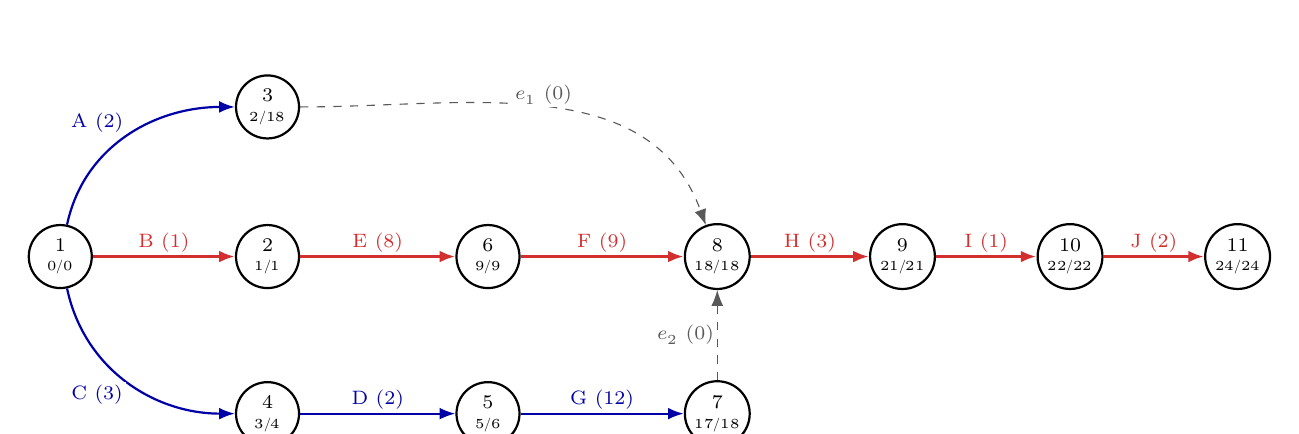
\begin{tikzpicture}[x=1.12cm,y=0.95cm]
  \node[event] (p1)  at (0.00,1.55) {1\\[-1pt]{\tiny $0/0$}};
  \node[event] (p3)  at (2.35,3.55) {3\\[-1pt]{\tiny $2/18$}};
  \node[event] (p2)  at (2.35,1.55) {2\\[-1pt]{\tiny $1/1$}};
  \node[event] (p4)  at (2.35,-0.55) {4\\[-1pt]{\tiny $3/4$}};
  \node[event] (p6)  at (4.85,1.55) {6\\[-1pt]{\tiny $9/9$}};
  \node[event] (p5)  at (4.85,-0.55) {5\\[-1pt]{\tiny $5/6$}};
  \node[event] (p8)  at (7.45,1.55) {8\\[-1pt]{\tiny $18/18$}};
  \node[event] (p7)  at (7.45,-0.55) {7\\[-1pt]{\tiny $17/18$}};
  \node[event] (p9)  at (9.55,1.55) {9\\[-1pt]{\tiny $21/21$}};
  \node[event] (p10) at (11.45,1.55) {10\\[-1pt]{\tiny $22/22$}};
  \node[event] (p11) at (13.35,1.55) {11\\[-1pt]{\tiny $24/24$}};

  \draw[arc] (p1) to[out=78,in=180] node[arclabel,above left] {A (2)} (p3);
  \draw[criticalarc] (p1) -- node[arclabel,above] {B (1)} (p2);
  \draw[arc] (p1) to[out=-78,in=180] node[arclabel,below left] {C (3)} (p4);
  \draw[criticalarc] (p2) -- node[arclabel,above] {E (8)} (p6);
  \draw[arc] (p4) -- node[arclabel,above] {D (2)} (p5);
  \draw[arc] (p5) -- node[arclabel,above] {G (12)} (p7);
  \draw[criticalarc] (p6) -- node[arclabel,above] {F (9)} (p8);
  \draw[dummyarc] (p3) to[out=0,in=110] node[arclabel,above] {$e_1$ (0)} (p8);
  \draw[dummyarc] (p7) -- node[arclabel,left] {$e_2$ (0)} (p8);
  \draw[criticalarc] (p8) -- node[arclabel,above] {H (3)} (p9);
  \draw[criticalarc] (p9) -- node[arclabel,above] {I (1)} (p10);
  \draw[criticalarc] (p10) -- node[arclabel,above] {J (2)} (p11);
\end{tikzpicture}}
\caption{Mạng PERT của Bài tập 2}
\end{figure}

{\small
\textbf{Tiến:}
$t_s(1)=0$,
$t_s(2)=1$,
$t_s(3)=2$,
$t_s(4)=3$,
$t_s(5)=5$,
$t_s(6)=9$,
$t_s(7)=17$,
$t_s(8)=\max\{2,18,17\}=18$,
$t_s(9)=21$,
$t_s(10)=22$,
$t_s(11)=24$.
\\
\textbf{Lùi:}
$t_m(11)=24$,
$t_m(10)=22$,
$t_m(9)=21$,
$t_m(8)=18$,
$t_m(7)=18$,
$t_m(6)=9$,
$t_m(5)=6$,
$t_m(4)=4$,
$t_m(3)=18$,
$t_m(2)=1$,
$t_m(1)=\min\{16,0,1\}=0$.
}

\begin{table}[H]\centering
\caption{Thời điểm sớm, muộn và dự trữ các sự kiện - Bài tập 2}
\begin{tabular}{c|rrrrrrrrrrr}
\toprule
Sự kiện & 1&2&3&4&5&6&7&8&9&10&11\\
\midrule
$t_s$ & 0&1&2&3&5&9&17&18&21&22&24\\
$t_m$ & 0&1&18&4&6&9&18&18&21&22&24\\
$R$   & 0&0&16&1&1&0&1&0&0&0&0\\
\bottomrule
\end{tabular}
\end{table}

Đỉnh găng: $1,2,6,8,9,10,11$. Thời gian sớm nhất hoàn thành dự án là \textbf{24 ngày}.

\subsection{Tính dự trữ và đường găng}

\begin{longtable}{c|c|r|rr|rr|rrr}
\caption{Các chỉ tiêu thời gian của công việc - Bài tập 2}\\
\toprule
\textbf{CV}&\textbf{$i\rightarrow j$}&\textbf{$d$}&\textbf{ES}&\textbf{EF}&\textbf{LS}&\textbf{LF}&\textbf{TF}&\textbf{FF}&\textbf{IF}\\
\midrule
\endfirsthead
\toprule
\textbf{CV}&\textbf{$i\rightarrow j$}&\textbf{$d$}&\textbf{ES}&\textbf{EF}&\textbf{LS}&\textbf{LF}&\textbf{TF}&\textbf{FF}&\textbf{IF}\\
\midrule
\endhead
A&$1\rightarrow 3$&2&0&2&16&18&16&0&0\\
B&$1\rightarrow 2$&1&0&1&0&1&0&0&0\\
C&$1\rightarrow 4$&3&0&3&1&4&1&0&0\\
D&$4\rightarrow 5$&2&3&5&4&6&1&0&0\\
E&$2\rightarrow 6$&8&1&9&1&9&0&0&0\\
F&$6\rightarrow 8$&9&9&18&9&18&0&0&0\\
G&$5\rightarrow 7$&12&5&17&6&18&1&0&0\\
H&$8\rightarrow 9$&3&18&21&18&21&0&0&0\\
I&$9\rightarrow 10$&1&21&22&21&22&0&0&0\\
J&$10\rightarrow 11$&2&22&24&22&24&0&0&0\\
\bottomrule
\end{longtable}

Đường găng gồm các công việc có $TF=0$:
\[
  \boxed{B-E-F-H-I-J\qquad (1+8+9+3+1+2=24\ \text{ngày})}.
\]
Đối chiếu: $A$-$H$-$I$-$J=8$; $C$-$D$-$G$-$H$-$I$-$J=23$.

Các công việc không găng là $A$ ($TF=16$) và $C,D,G$ ($TF=1$).
Mọi công việc đều có $IF=0$, nên không thể đồng thời kéo dài tất cả công việc không găng thêm ngày nào mà không ảnh hưởng tiến độ: chuỗi $C$-$D$-$G$ chỉ còn 1 ngày dự trữ chung.

\subsection{Biểu đồ Gantt}

\begin{figure}[H]\centering
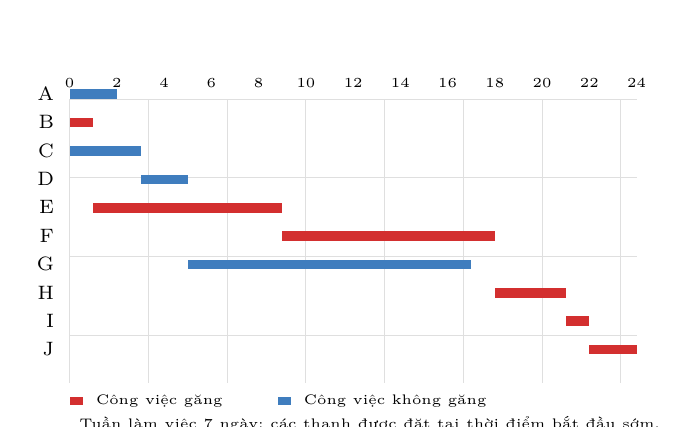
\begin{tikzpicture}[x=0.30cm,y=0.36cm]
  \draw[gray!25] (0,0) grid (24,-10);
  \foreach \x in {0,2,...,24} \node[font=\tiny,anchor=south] at (\x,0.05) {\x};
  \ganttrowseven{0}{A}{0}{2}{normalbar}
  \ganttrowseven{1}{B}{0}{1}{criticalbar}
  \ganttrowseven{2}{C}{0}{3}{normalbar}
  \ganttrowseven{3}{D}{3}{2}{normalbar}
  \ganttrowseven{4}{E}{1}{8}{criticalbar}
  \ganttrowseven{5}{F}{9}{9}{criticalbar}
  \ganttrowseven{6}{G}{5}{12}{normalbar}
  \ganttrowseven{7}{H}{18}{3}{criticalbar}
  \ganttrowseven{8}{I}{21}{1}{criticalbar}
  \ganttrowseven{9}{J}{22}{2}{criticalbar}
  \ganttlegend{10.8}
  \node[font=\tiny,anchor=west] at (0,-11.45) {Tuần làm việc 7 ngày; các thanh được đặt tại thời điểm bắt đầu sớm.};
\end{tikzpicture}
\caption{Gantt Bài tập 2 - lịch 7 ngày}
\end{figure}

\begin{figure}[H]\centering
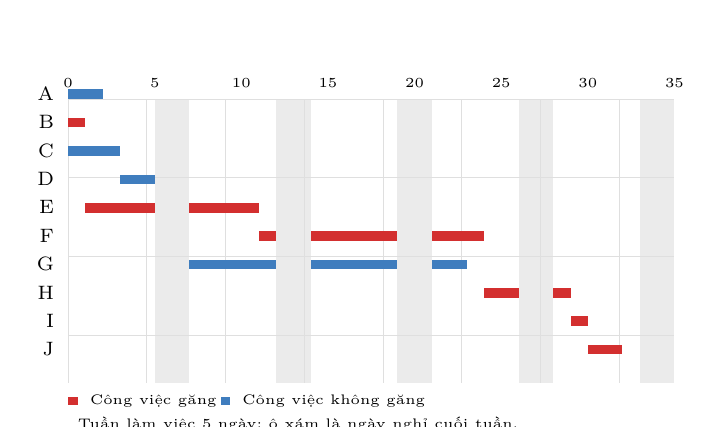
\begin{tikzpicture}[x=0.22cm,y=0.36cm]
  \foreach \w in {0,1,2,3,4} {\fill[weekend] ({7*\w+5},0) rectangle ({7*\w+7},-10);}
  \draw[gray!25] (0,0) grid (35,-10);
  \foreach \x in {0,5,...,35} \node[font=\tiny,anchor=south] at (\x,0.05) {\x};
  \ganttrowfive{0}{A}{0}{2}{normalbar}
  \ganttrowfive{1}{B}{0}{1}{criticalbar}
  \ganttrowfive{2}{C}{0}{3}{normalbar}
  \ganttrowfive{3}{D}{3}{2}{normalbar}
  \ganttrowfive{4}{E}{1}{8}{criticalbar}
  \ganttrowfive{5}{F}{9}{9}{criticalbar}
  \ganttrowfive{6}{G}{5}{12}{normalbar}
  \ganttrowfive{7}{H}{18}{3}{criticalbar}
  \ganttrowfive{8}{I}{21}{1}{criticalbar}
  \ganttrowfive{9}{J}{22}{2}{criticalbar}
  \ganttlegend{10.8}
  \node[font=\tiny,anchor=west] at (0,-11.45) {Tuần làm việc 5 ngày; ô xám là ngày nghỉ cuối tuần.};
\end{tikzpicture}
\caption{Gantt Bài tập 2 - lịch 5 ngày}
\end{figure}

\clearpage
\section{Bài tập 3}

\subsection{Dữ liệu}

\begin{table}[H]\centering
\caption{Dữ liệu công việc của Bài tập 3}
\begin{tabular}{c c c}
\toprule
\textbf{Công việc} & \textbf{Trình tự} & \textbf{Thời gian (ngày)}\\
\midrule
A & Từ đầu & 3\\
B & Từ đầu & 4\\
C & Từ đầu & 4\\
D & Sau A & 5\\
G & Sau D & 5\\
H & Sau A & 9\\
F & Sau B, G & 7\\
I & Sau C & 6\\
K & Sau F & 3\\
L & Sau F & 10\\
M & Sau F, I & 9\\
N & Sau H, K & 7\\
P & Sau L, M, N & 12\\
\bottomrule
\end{tabular}
\end{table}

\subsection{Sơ đồ PERT và chỉ tiêu sự kiện}

\begin{figure}[H]\centering
\resizebox{\linewidth}{!}{%
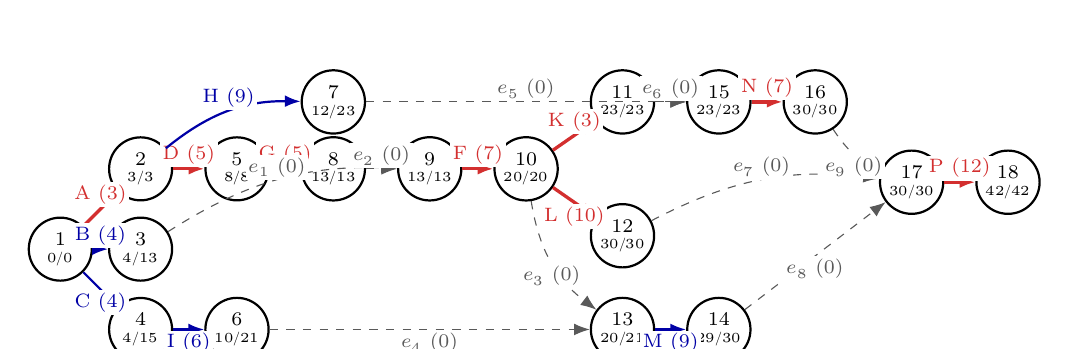
\begin{tikzpicture}[x=1.02cm,y=0.85cm]
  \node[event] (p1) at (0,2) {1\\[-2pt]\tiny $0/0$};
  \node[event] (p2) at (1,3.2) {2\\[-2pt]\tiny $3/3$};
  \node[event] (p3) at (1,2) {3\\[-2pt]\tiny $4/13$};
  \node[event] (p4) at (1,0.8) {4\\[-2pt]\tiny $4/15$};
  \node[event] (p5) at (2.2,3.2) {5\\[-2pt]\tiny $8/8$};
  \node[event] (p6) at (2.2,0.8) {6\\[-2pt]\tiny $10/21$};
  \node[event] (p7) at (3.4,4.2) {7\\[-2pt]\tiny $12/23$};
  \node[event] (p8) at (3.4,3.2) {8\\[-2pt]\tiny $13/13$};
  \node[event] (p9) at (4.6,3.2) {9\\[-2pt]\tiny $13/13$};
  \node[event] (p10) at (5.8,3.2) {10\\[-2pt]\tiny $20/20$};
  \node[event] (p11) at (7.0,4.2) {11\\[-2pt]\tiny $23/23$};
  \node[event] (p12) at (7.0,2.2) {12\\[-2pt]\tiny $30/30$};
  \node[event] (p13) at (7.0,0.8) {13\\[-2pt]\tiny $20/21$};
  \node[event] (p14) at (8.2,0.8) {14\\[-2pt]\tiny $29/30$};
  \node[event] (p15) at (8.2,4.2) {15\\[-2pt]\tiny $23/23$};
  \node[event] (p16) at (9.4,4.2) {16\\[-2pt]\tiny $30/30$};
  \node[event] (p17) at (10.6,3.0) {17\\[-2pt]\tiny $30/30$};
  \node[event] (p18) at (11.8,3.0) {18\\[-2pt]\tiny $42/42$};
  \draw[criticalarc] (p1) -- node[arclabel,above] {A (3)} (p2);
  \draw[arc] (p1) -- node[arclabel,above] {B (4)} (p3);
  \draw[arc] (p1) -- node[arclabel,below] {C (4)} (p4);
  \draw[criticalarc] (p2) -- node[arclabel,above] {D (5)} (p5);
  \draw[arc] (p4) -- node[arclabel,below] {I (6)} (p6);
  \draw[arc] (p2) to[bend left=20] node[arclabel,above] {H (9)} (p7);
  \draw[criticalarc] (p5) -- node[arclabel,above] {G (5)} (p8);
  \draw[dummyarc] (p3) to[bend left=17] node[arclabel,above] {$e_1$ (0)} (p9);
  \draw[dummyarc] (p8) -- node[arclabel,above] {$e_2$ (0)} (p9);
  \draw[criticalarc] (p9) -- node[arclabel,above] {F (7)} (p10);
  \draw[criticalarc] (p10) -- node[arclabel,above] {K (3)} (p11);
  \draw[criticalarc] (p10) -- node[arclabel,below] {L (10)} (p12);
  \draw[dummyarc] (p10) to[bend right=22] node[arclabel,below] {$e_3$ (0)} (p13);
  \draw[dummyarc] (p6) -- node[arclabel,below] {$e_4$ (0)} (p13);
  \draw[arc] (p13) -- node[arclabel,below] {M (9)} (p14);
  \draw[dummyarc] (p7) -- node[arclabel,above] {$e_5$ (0)} (p15);
  \draw[dummyarc] (p11) -- node[arclabel,above] {$e_6$ (0)} (p15);
  \draw[criticalarc] (p15) -- node[arclabel,above] {N (7)} (p16);
  \draw[dummyarc] (p12) to[bend left=17] node[arclabel,above] {$e_7$ (0)} (p17);
  \draw[dummyarc] (p14) -- node[arclabel,below] {$e_8$ (0)} (p17);
  \draw[dummyarc] (p16) to[bend right=17] node[arclabel,below] {$e_9$ (0)} (p17);
  \draw[criticalarc] (p17) -- node[arclabel,above] {P (12)} (p18);
\end{tikzpicture}}
\caption{Mạng PERT của Bài tập 3}
\end{figure}

\begin{table}[H]\centering
\caption{Thời điểm sớm và muộn của các sự kiện - Bài tập 3}
\scriptsize
\begin{tabular}{c|rrrrrrrrrrrrrrrrrr}
\toprule
Sự kiện&1&2&3&4&5&6&7&8&9&10&11&12&13&14&15&16&17&18\\
\midrule
$t_s$&0&3&4&4&8&10&12&13&13&20&23&30&20&29&23&30&30&42\\
$t_m$&0&3&13&15&8&21&23&13&13&20&23&30&21&30&23&30&30&42\\
\bottomrule
\end{tabular}
\end{table}

\subsection{Tính dự trữ và đường găng}

\begin{longtable}{c|r|rr|rr|rrr}
\caption{Các chỉ tiêu thời gian của công việc - Bài tập 3}\\
\toprule
\textbf{CV}&\textbf{$d$}&\textbf{ES}&\textbf{EF}&\textbf{LS}&\textbf{LF}&\textbf{TF}&\textbf{FF}&\textbf{IF}\\
\midrule
\endfirsthead
\toprule
\textbf{CV}&\textbf{$d$}&\textbf{ES}&\textbf{EF}&\textbf{LS}&\textbf{LF}&\textbf{TF}&\textbf{FF}&\textbf{IF}\\
\midrule
\endhead
A&3&0&3&0&3&0&0&0\\
B&4&0&4&9&13&9&0&0\\
C&4&0&4&11&15&11&0&0\\
D&5&3&8&3&8&0&0&0\\
G&5&8&13&8&13&0&0&0\\
H&9&3&12&14&23&11&0&0\\
F&7&13&20&13&20&0&0&0\\
I&6&4&10&15&21&11&0&0\\
K&3&20&23&20&23&0&0&0\\
L&10&20&30&20&30&0&0&0\\
M&9&20&29&21&30&1&0&0\\
N&7&23&30&23&30&0&0&0\\
P&12&30&42&30&42&0&0&0\\
\bottomrule
\end{longtable}

Thời gian ngắn nhất của dự án là \textbf{42 ngày}. Do có hai nhánh cùng đạt
thời gian lớn nhất, dự án có hai đường găng:
\[
\boxed{A-D-G-F-L-P}
\qquad\text{và}\qquad
\boxed{A-D-G-F-K-N-P}.
\]
Các công việc không găng là $B,C,H,I,M$; $TF$ tương ứng là 9, 11, 11, 11
và 1 ngày. Mức kéo dài đồng thời lớn nhất của tất cả công việc không găng là
\textbf{1 ngày}. Các $IF$ của công việc không găng đều bằng 0.

\subsection{Biểu đồ Gantt}

\begin{figure}[H]\centering
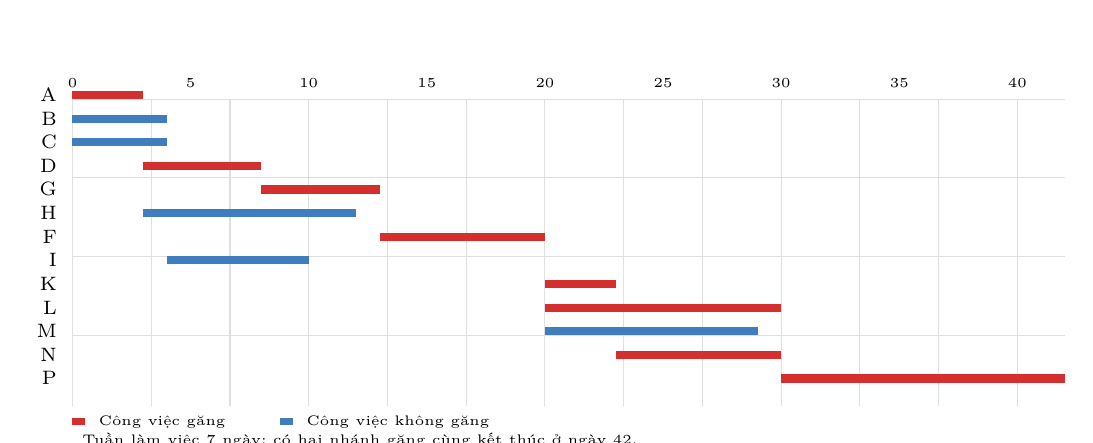
\begin{tikzpicture}[x=0.30cm,y=0.30cm]
  \draw[gray!25] (0,0) grid (42,-13);
  \foreach \x in {0,5,...,40} \node[font=\tiny,anchor=south] at (\x,0.05) {\x};
  \ganttrowseven{0}{A}{0}{3}{criticalbar}
  \ganttrowseven{1}{B}{0}{4}{normalbar}
  \ganttrowseven{2}{C}{0}{4}{normalbar}
  \ganttrowseven{3}{D}{3}{5}{criticalbar}
  \ganttrowseven{4}{G}{8}{5}{criticalbar}
  \ganttrowseven{5}{H}{3}{9}{normalbar}
  \ganttrowseven{6}{F}{13}{7}{criticalbar}
  \ganttrowseven{7}{I}{4}{6}{normalbar}
  \ganttrowseven{8}{K}{20}{3}{criticalbar}
  \ganttrowseven{9}{L}{20}{10}{criticalbar}
  \ganttrowseven{10}{M}{20}{9}{normalbar}
  \ganttrowseven{11}{N}{23}{7}{criticalbar}
  \ganttrowseven{12}{P}{30}{12}{criticalbar}
  \ganttlegend{13.8}
  \node[font=\tiny,anchor=west] at (0,-14.45) {Tuần làm việc 7 ngày; có hai nhánh găng cùng kết thúc ở ngày 42.};
\end{tikzpicture}
\caption{Gantt Bài tập 3 - lịch 7 ngày}
\end{figure}

\begin{figure}[H]\centering
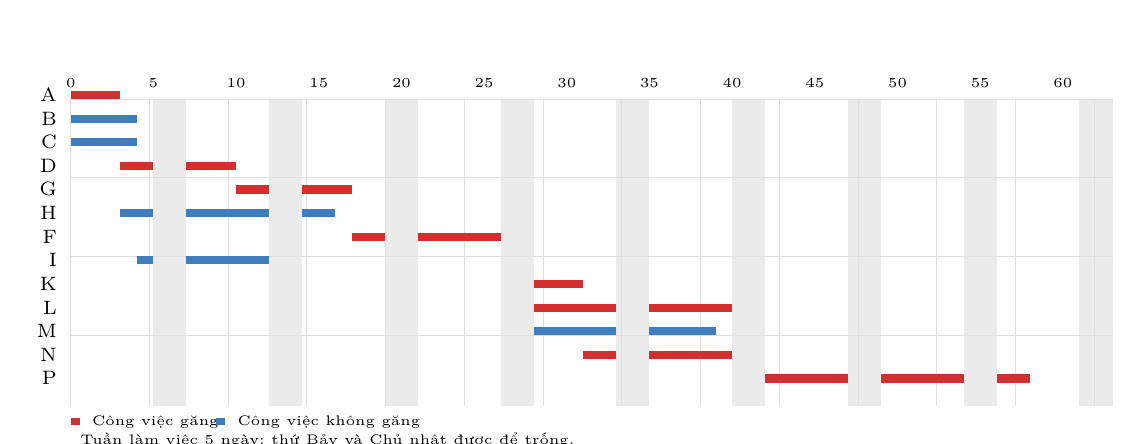
\begin{tikzpicture}[x=0.21cm,y=0.30cm]
  \foreach \w in {0,1,2,3,4,5,6,7,8} {\fill[weekend] ({7*\w+5},0) rectangle ({7*\w+7},-13);}
  \draw[gray!25] (0,0) grid (63,-13);
  \foreach \x in {0,5,...,60} \node[font=\tiny,anchor=south] at (\x,0.05) {\x};
  \ganttrowfive{0}{A}{0}{3}{criticalbar}
  \ganttrowfive{1}{B}{0}{4}{normalbar}
  \ganttrowfive{2}{C}{0}{4}{normalbar}
  \ganttrowfive{3}{D}{3}{5}{criticalbar}
  \ganttrowfive{4}{G}{8}{5}{criticalbar}
  \ganttrowfive{5}{H}{3}{9}{normalbar}
  \ganttrowfive{6}{F}{13}{7}{criticalbar}
  \ganttrowfive{7}{I}{4}{6}{normalbar}
  \ganttrowfive{8}{K}{20}{3}{criticalbar}
  \ganttrowfive{9}{L}{20}{10}{criticalbar}
  \ganttrowfive{10}{M}{20}{9}{normalbar}
  \ganttrowfive{11}{N}{23}{7}{criticalbar}
  \ganttrowfive{12}{P}{30}{12}{criticalbar}
  \ganttlegend{13.8}
  \node[font=\tiny,anchor=west] at (0,-14.45) {Tuần làm việc 5 ngày; thứ Bảy và Chủ nhật được để trống.};
\end{tikzpicture}
\caption{Gantt Bài tập 3 - lịch 5 ngày}
\end{figure}

\clearpage
\section{Bài tập 4}

\subsection{Dữ liệu}

\begin{table}[H]\centering
\caption{Dữ liệu công việc của Bài tập 4}
\begin{tabular}{c c c}
\toprule
\textbf{Công việc} & \textbf{Trình tự} & \textbf{Thời gian (ngày)}\\
\midrule
A & Từ đầu & 3\\
B & Từ đầu & 2\\
C & Sau A & 4\\
D & Sau A & 2\\
G & Sau C & 3\\
H & Sau B, D, G & 6\\
F & Sau C & 9\\
I & Sau H & 5\\
K & Sau I & 6\\
L & Sau I & 5\\
M & Sau F, K, L & 7\\
N & Sau F, K & 10\\
\bottomrule
\end{tabular}
\end{table}

\subsection{Sơ đồ PERT và chỉ tiêu sự kiện}

\begin{figure}[H]\centering
\resizebox{0.99\linewidth}{!}{%
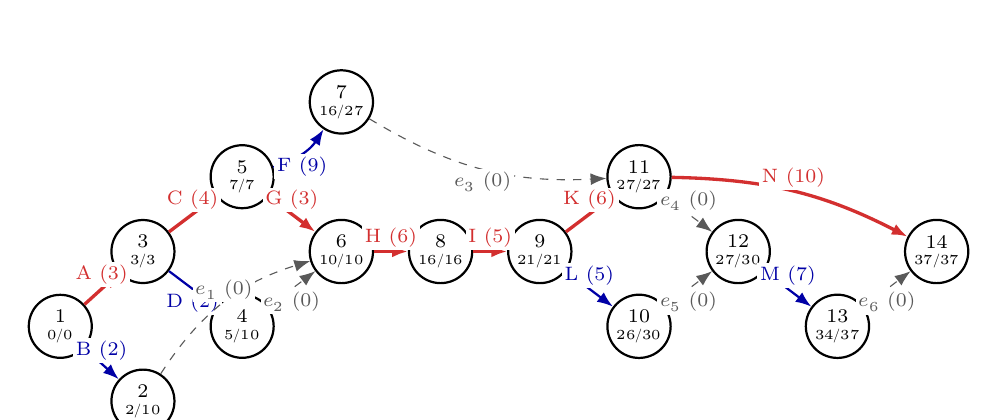
\begin{tikzpicture}[x=1.05cm,y=0.95cm]
  \node[event] (p1) at (0,1) {1\\[-2pt]\tiny $0/0$};
  \node[event] (p2) at (1,0) {2\\[-2pt]\tiny $2/10$};
  \node[event] (p3) at (1,2) {3\\[-2pt]\tiny $3/3$};
  \node[event] (p4) at (2.2,1) {4\\[-2pt]\tiny $5/10$};
  \node[event] (p5) at (2.2,3) {5\\[-2pt]\tiny $7/7$};
  \node[event] (p6) at (3.4,2) {6\\[-2pt]\tiny $10/10$};
  \node[event] (p7) at (3.4,4) {7\\[-2pt]\tiny $16/27$};
  \node[event] (p8) at (4.6,2) {8\\[-2pt]\tiny $16/16$};
  \node[event] (p9) at (5.8,2) {9\\[-2pt]\tiny $21/21$};
  \node[event] (p10) at (7.0,1) {10\\[-2pt]\tiny $26/30$};
  \node[event] (p11) at (7.0,3) {11\\[-2pt]\tiny $27/27$};
  \node[event] (p12) at (8.2,2) {12\\[-2pt]\tiny $27/30$};
  \node[event] (p13) at (9.4,1) {13\\[-2pt]\tiny $34/37$};
  \node[event] (p14) at (10.6,2) {14\\[-2pt]\tiny $37/37$};
  \draw[criticalarc] (p1) -- node[arclabel,above] {A (3)} (p3);
  \draw[arc] (p1) -- node[arclabel,above] {B (2)} (p2);
  \draw[criticalarc] (p3) -- node[arclabel,above] {C (4)} (p5);
  \draw[arc] (p3) -- node[arclabel,below] {D (2)} (p4);
  \draw[criticalarc] (p5) -- node[arclabel,above] {G (3)} (p6);
  \draw[dummyarc] (p2) to[bend left=20] node[arclabel,above] {$e_1$ (0)} (p6);
  \draw[dummyarc] (p4) -- node[arclabel,below] {$e_2$ (0)} (p6);
  \draw[criticalarc] (p6) -- node[arclabel,above] {H (6)} (p8);
  \draw[arc] (p5) to[bend right=20] node[arclabel,below] {F (9)} (p7);
  \draw[criticalarc] (p8) -- node[arclabel,above] {I (5)} (p9);
  \draw[arc] (p9) -- node[arclabel,above] {L (5)} (p10);
  \draw[criticalarc] (p9) -- node[arclabel,above] {K (6)} (p11);
  \draw[dummyarc] (p7) to[bend right=17] node[arclabel,below] {$e_3$ (0)} (p11);
  \draw[dummyarc] (p11) -- node[arclabel,above] {$e_4$ (0)} (p12);
  \draw[dummyarc] (p10) -- node[arclabel,below] {$e_5$ (0)} (p12);
  \draw[arc] (p12) -- node[arclabel,above] {M (7)} (p13);
  \draw[criticalarc] (p11) to[bend left=13] node[arclabel,above] {N (10)} (p14);
  \draw[dummyarc] (p13) -- node[arclabel,below] {$e_6$ (0)} (p14);
\end{tikzpicture}}
\caption{Mạng PERT của Bài tập 4}
\end{figure}

\begin{table}[H]\centering
\caption{Thời điểm sớm và muộn của các sự kiện - Bài tập 4}
\begin{tabular}{c|rrrrrrrrrrrrrr}
\toprule
Sự kiện&1&2&3&4&5&6&7&8&9&10&11&12&13&14\\
\midrule
$t_s$&0&2&3&5&7&10&16&16&21&26&27&27&34&37\\
$t_m$&0&10&3&10&7&10&27&16&21&30&27&30&37&37\\
\bottomrule
\end{tabular}
\end{table}

\subsection{Tính dự trữ và đường găng}

\begin{longtable}{c|r|rr|rr|rrr}
\caption{Các chỉ tiêu thời gian của công việc - Bài tập 4}\\
\toprule
\textbf{CV}&\textbf{$d$}&\textbf{ES}&\textbf{EF}&\textbf{LS}&\textbf{LF}&\textbf{TF}&\textbf{FF}&\textbf{IF}\\
\midrule
\endfirsthead
\toprule
\textbf{CV}&\textbf{$d$}&\textbf{ES}&\textbf{EF}&\textbf{LS}&\textbf{LF}&\textbf{TF}&\textbf{FF}&\textbf{IF}\\
\midrule
\endhead
A&3&0&3&0&3&0&0&0\\
B&2&0&2&8&10&8&0&0\\
C&4&3&7&3&7&0&0&0\\
D&2&3&5&8&10&5&0&0\\
G&3&7&10&7&10&0&0&0\\
H&6&10&16&10&16&0&0&0\\
F&9&7&16&18&27&11&0&0\\
I&5&16&21&16&21&0&0&0\\
K&6&21&27&21&27&0&0&0\\
L&5&21&26&25&30&4&0&0\\
M&7&27&34&30&37&3&0&0\\
N&10&27&37&27&37&0&0&0\\
\bottomrule
\end{longtable}

Thời gian ngắn nhất của dự án là \textbf{37 ngày}. Đường găng là
\[
  \boxed{A-C-G-H-I-K-N}.
\]
Các công việc không găng là $B,D,F,L,M$, có $TF$ lần lượt là 8, 5, 11,
4 và 3 ngày. Vì vậy, tất cả các công việc không găng có thể đồng thời kéo
dài tối đa \textbf{3 ngày} mà không làm thay đổi tiến độ dự án. Các công việc
không găng có $IF=0$ theo công thức PERT độc lập.

\subsection{Biểu đồ Gantt}

\begin{figure}[H]\centering
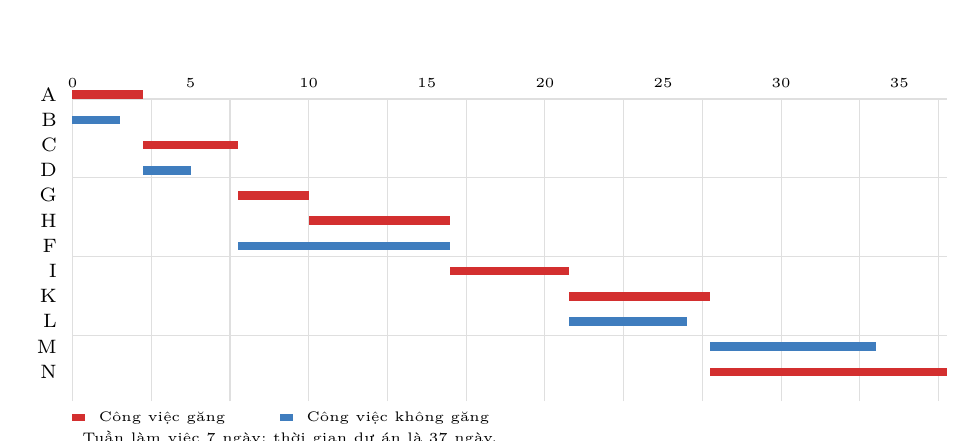
\begin{tikzpicture}[x=0.30cm,y=0.32cm]
  \draw[gray!25] (0,0) grid (37,-12);
  \foreach \x in {0,5,...,35} \node[font=\tiny,anchor=south] at (\x,0.05) {\x};
  \ganttrowseven{0}{A}{0}{3}{criticalbar}
  \ganttrowseven{1}{B}{0}{2}{normalbar}
  \ganttrowseven{2}{C}{3}{4}{criticalbar}
  \ganttrowseven{3}{D}{3}{2}{normalbar}
  \ganttrowseven{4}{G}{7}{3}{criticalbar}
  \ganttrowseven{5}{H}{10}{6}{criticalbar}
  \ganttrowseven{6}{F}{7}{9}{normalbar}
  \ganttrowseven{7}{I}{16}{5}{criticalbar}
  \ganttrowseven{8}{K}{21}{6}{criticalbar}
  \ganttrowseven{9}{L}{21}{5}{normalbar}
  \ganttrowseven{10}{M}{27}{7}{normalbar}
  \ganttrowseven{11}{N}{27}{10}{criticalbar}
  \ganttlegend{12.8}
  \node[font=\tiny,anchor=west] at (0,-13.45) {Tuần làm việc 7 ngày; thời gian dự án là 37 ngày.};
\end{tikzpicture}
\caption{Gantt Bài tập 4 - lịch 7 ngày}
\end{figure}

\begin{figure}[H]\centering
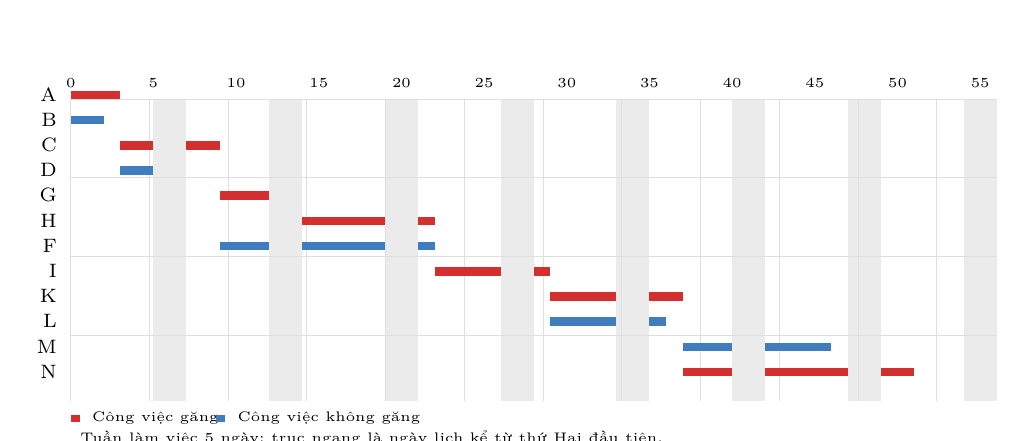
\begin{tikzpicture}[x=0.21cm,y=0.32cm]
  \foreach \w in {0,1,2,3,4,5,6,7} {\fill[weekend] ({7*\w+5},0) rectangle ({7*\w+7},-12);}
  \draw[gray!25] (0,0) grid (56,-12);
  \foreach \x in {0,5,...,55} \node[font=\tiny,anchor=south] at (\x,0.05) {\x};
  \ganttrowfive{0}{A}{0}{3}{criticalbar}
  \ganttrowfive{1}{B}{0}{2}{normalbar}
  \ganttrowfive{2}{C}{3}{4}{criticalbar}
  \ganttrowfive{3}{D}{3}{2}{normalbar}
  \ganttrowfive{4}{G}{7}{3}{criticalbar}
  \ganttrowfive{5}{H}{10}{6}{criticalbar}
  \ganttrowfive{6}{F}{7}{9}{normalbar}
  \ganttrowfive{7}{I}{16}{5}{criticalbar}
  \ganttrowfive{8}{K}{21}{6}{criticalbar}
  \ganttrowfive{9}{L}{21}{5}{normalbar}
  \ganttrowfive{10}{M}{27}{7}{normalbar}
  \ganttrowfive{11}{N}{27}{10}{criticalbar}
  \ganttlegend{12.8}
  \node[font=\tiny,anchor=west] at (0,-13.45) {Tuần làm việc 5 ngày; trục ngang là ngày lịch kể từ thứ Hai đầu tiên.};
\end{tikzpicture}
\caption{Gantt Bài tập 4 - lịch 5 ngày}
\end{figure}

\clearpage
\section{Bài tập 5}

\subsection{Dữ liệu}

\begin{table}[H]\centering
\caption{Dữ liệu công việc của Bài tập 5}
\begin{tabular}{c c c}
\toprule
\textbf{Công việc} & \textbf{Trình tự} & \textbf{Thời gian (ngày)}\\
\midrule
A & Từ đầu & 2\\
B & Từ đầu & 6\\
C & Sau A & 3\\
D & Sau B, C & 4\\
G & Sau A & 5\\
H & Sau D, G & 5\\
F & Sau D & 4\\
I & Sau B, C & 7\\
K & Sau H, F & 6\\
L & Sau I & 6\\
\bottomrule
\end{tabular}
\end{table}

\subsection{Sơ đồ PERT và chỉ tiêu sự kiện}

\begin{figure}[H]\centering
\resizebox{0.99\linewidth}{!}{%
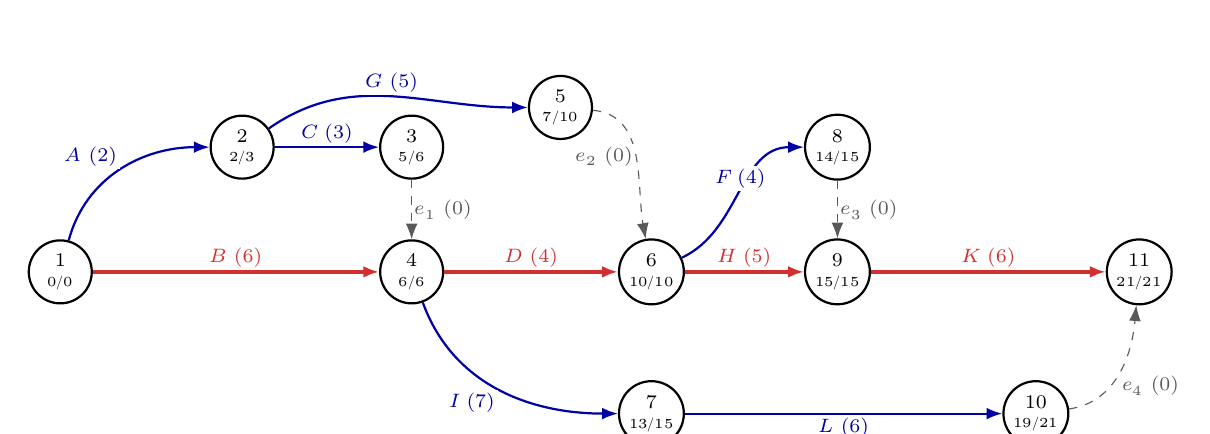
\begin{tikzpicture}[x=1.05cm,y=0.72cm]
  \node[event] (p1)  at (0.00, 2.15) {1\\[-1pt]{\tiny\normalfont $0/0$}};
  \node[event] (p2)  at (2.20, 4.35) {2\\[-1pt]{\tiny\normalfont $2/3$}};
  \node[event] (p3)  at (4.25, 4.35) {3\\[-1pt]{\tiny\normalfont $5/6$}};
  \node[event] (p4)  at (4.25, 2.15) {4\\[-1pt]{\tiny\normalfont $6/6$}};
  \node[event] (p5)  at (6.05, 5.05) {5\\[-1pt]{\tiny\normalfont $7/10$}};
  \node[event] (p6)  at (7.15, 2.15) {6\\[-1pt]{\tiny\normalfont $10/10$}};
  \node[event] (p7)  at (7.15,-0.35) {7\\[-1pt]{\tiny\normalfont $13/15$}};
  \node[event] (p8)  at (9.40, 4.35) {8\\[-1pt]{\tiny\normalfont $14/15$}};
  \node[event] (p9)  at (9.40, 2.15) {9\\[-1pt]{\tiny\normalfont $15/15$}};
  \node[event] (p10) at (11.80,-0.35) {10\\[-1pt]{\tiny\normalfont $19/21$}};
  \node[event] (p11) at (13.05, 2.15) {11\\[-1pt]{\tiny\normalfont $21/21$}};
  \draw[arc] (p1) to[out=75,in=180] node[arclabel,above left] {$A$ (2)} (p2);
  \draw[criticalarc] (p1) -- node[arclabel,above] {$B$ (6)} (p4);
  \draw[arc] (p2) -- node[arclabel,above] {$C$ (3)} (p3);
  \draw[dummyarc] (p3) -- node[arclabel,right] {$e_1$ (0)} (p4);
  \draw[arc] (p2) to[out=35,in=180] node[arclabel,above] {$G$ (5)} (p5);
  \draw[dummyarc] (p5) to[out=-5,in=100] node[arclabel,left] {$e_2$ (0)} (p6);
  \draw[criticalarc] (p4) -- node[arclabel,above] {$D$ (4)} (p6);
  \draw[arc] (p4) to[out=-70,in=180] node[arclabel,below left] {$I$ (7)} (p7);
  \draw[criticalarc] (p6) -- node[arclabel,above] {$H$ (5)} (p9);
  \draw[arc] (p6) to[out=25,in=180] node[arclabel,above] {$F$ (4)} (p8);
  \draw[dummyarc] (p8) -- node[arclabel,right] {$e_3$ (0)} (p9);
  \draw[arc] (p7) -- node[arclabel,below] {$L$ (6)} (p10);
  \draw[criticalarc] (p9) -- node[arclabel,above] {$K$ (6)} (p11);
  \draw[dummyarc] (p10) to[out=8,in=-95] node[arclabel,below right] {$e_4$ (0)} (p11);
\end{tikzpicture}}
\caption{Mạng PERT của Bài tập 5. Đường găng $B$--$D$--$H$--$K$.}
\end{figure}

\begin{table}[H]\centering
\caption{Thời điểm sớm và muộn của các sự kiện - Bài tập 5}
\begin{tabular}{c|rrrrrrrrrrr}
\toprule
Sự kiện&1&2&3&4&5&6&7&8&9&10&11\\
\midrule
$t_s$&0&2&5&6&7&10&13&14&15&19&21\\
$t_m$&0&3&6&6&10&10&15&15&15&21&21\\
$R$&0&1&1&0&3&0&2&1&0&2&0\\
\bottomrule
\end{tabular}
\end{table}

\subsection{Tính dự trữ và đường găng}

\begin{longtable}{c|r|rr|rr|rrr}
\caption{Các chỉ tiêu thời gian của công việc - Bài tập 5}\\
\toprule
\textbf{CV}&\textbf{$d$}&\textbf{ES}&\textbf{EF}&\textbf{LS}&\textbf{LF}&\textbf{TF}&\textbf{FF}&\textbf{IF}\\
\midrule
\endfirsthead
\toprule
\textbf{CV}&\textbf{$d$}&\textbf{ES}&\textbf{EF}&\textbf{LS}&\textbf{LF}&\textbf{TF}&\textbf{FF}&\textbf{IF}\\
\midrule
\endhead
A&2&0&2&1&3&1&0&0\\
B&6&0&6&0&6&0&0&0\\
C&3&2&5&3&6&1&0&0\\
D&4&6&10&6&10&0&0&0\\
G&5&2&7&5&10&3&0&0\\
H&5&10&15&10&15&0&0&0\\
F&4&10&14&11&15&1&0&0\\
I&7&6&13&8&15&2&0&0\\
K&6&15&21&15&21&0&0&0\\
L&6&13&19&15&21&2&0&0\\
\bottomrule
\end{longtable}

Thời gian ngắn nhất của dự án là \textbf{21 ngày}. Đỉnh găng: $1,4,6,9,11$.
Đường găng là
\[
  \boxed{B\text{--}D\text{--}H\text{--}K\qquad (6+4+5+6=21\ \text{ngày})}.
\]
Các công việc không găng là $A,C,G,F,I,L$, có $TF$ lần lượt là 1, 1, 3,
1, 2 và 2 ngày. Không lấy $\min TF=1$ làm mức kéo dài đồng thời, vì $A$ và
$C$ nằm cùng chuỗi $A$--$C$--$D$--$H$--$K$ dài $20+2x\le 21\Rightarrow x\le 0{,}5$.
Mức kéo dài đồng thời lớn nhất là \textbf{0,5 ngày}. Dự trữ độc lập PERT
của mọi công việc bằng 0.

\subsection{Biểu đồ Gantt}

\begin{figure}[H]\centering
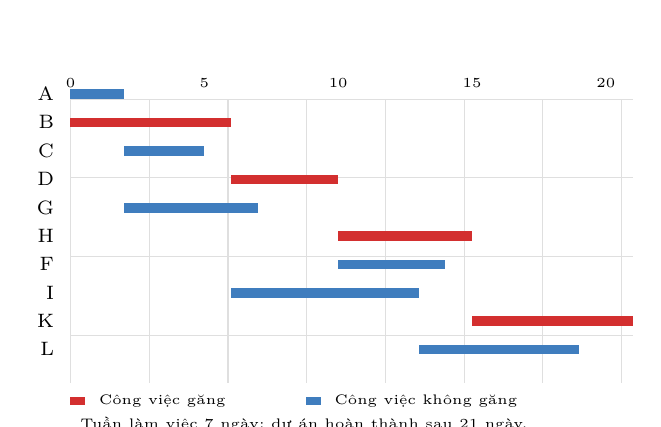
\begin{tikzpicture}[x=0.34cm,y=0.36cm]
  \draw[gray!25] (0,0) grid (21,-10);
  \foreach \x in {0,5,...,20} \node[font=\tiny,anchor=south] at (\x,0.05) {\x};
  \ganttrowseven{0}{A}{0}{2}{normalbar}
  \ganttrowseven{1}{B}{0}{6}{criticalbar}
  \ganttrowseven{2}{C}{2}{3}{normalbar}
  \ganttrowseven{3}{D}{6}{4}{criticalbar}
  \ganttrowseven{4}{G}{2}{5}{normalbar}
  \ganttrowseven{5}{H}{10}{5}{criticalbar}
  \ganttrowseven{6}{F}{10}{4}{normalbar}
  \ganttrowseven{7}{I}{6}{7}{normalbar}
  \ganttrowseven{8}{K}{15}{6}{criticalbar}
  \ganttrowseven{9}{L}{13}{6}{normalbar}
  \ganttlegend{10.8}
  \node[font=\tiny,anchor=west] at (0,-11.45) {Tuần làm việc 7 ngày; dự án hoàn thành sau 21 ngày.};
\end{tikzpicture}
\caption{Gantt Bài tập 5 - lịch 7 ngày}
\end{figure}

\begin{figure}[H]\centering
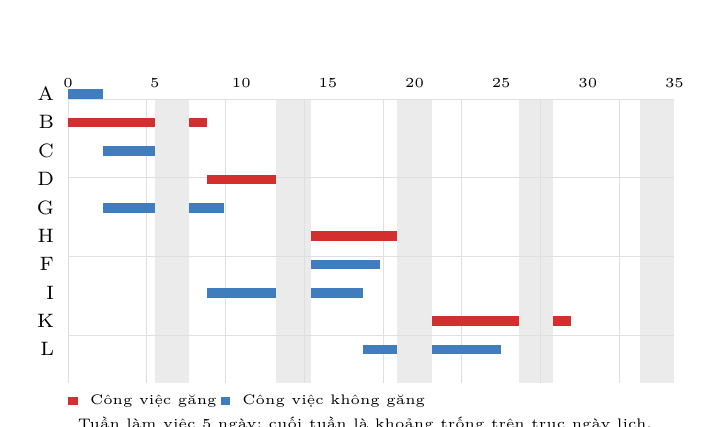
\begin{tikzpicture}[x=0.22cm,y=0.36cm]
  \foreach \w in {0,1,2,3,4} {\fill[weekend] ({7*\w+5},0) rectangle ({7*\w+7},-10);}
  \draw[gray!25] (0,0) grid (35,-10);
  \foreach \x in {0,5,...,35} \node[font=\tiny,anchor=south] at (\x,0.05) {\x};
  \ganttrowfive{0}{A}{0}{2}{normalbar}
  \ganttrowfive{1}{B}{0}{6}{criticalbar}
  \ganttrowfive{2}{C}{2}{3}{normalbar}
  \ganttrowfive{3}{D}{6}{4}{criticalbar}
  \ganttrowfive{4}{G}{2}{5}{normalbar}
  \ganttrowfive{5}{H}{10}{5}{criticalbar}
  \ganttrowfive{6}{F}{10}{4}{normalbar}
  \ganttrowfive{7}{I}{6}{7}{normalbar}
  \ganttrowfive{8}{K}{15}{6}{criticalbar}
  \ganttrowfive{9}{L}{13}{6}{normalbar}
  \ganttlegend{10.8}
  \node[font=\tiny,anchor=west] at (0,-11.45) {Tuần làm việc 5 ngày; cuối tuần là khoảng trống trên trục ngày lịch.};
\end{tikzpicture}
\caption{Gantt Bài tập 5 - lịch 5 ngày}
\end{figure}

\clearpage

\section{Tổng hợp kết quả}

\begin{table}[H]\centering
\caption{Tổng hợp thời gian và đường găng}
\small
\begin{tabular}{c|c|>{\centering\arraybackslash}p{7.2cm}|c}
\toprule
\textbf{Bài} & \textbf{Thời gian dự án} & \textbf{Đường găng} & \textbf{Kéo dài đồng thời}\\
\midrule
1 & 9 ngày & $A-B-D-H-I$ & 1 ngày\\
2 & 24 ngày & $B-E-F-H-I-J$ & 0 ngày\\
3 & 42 ngày & \parbox[c]{7.2cm}{\centering $A-D-G-F-L-P$;\\[-1pt] $A-D-G-F-K-N-P$} & 1 ngày\\
4 & 37 ngày & $A-C-G-H-I-K-N$ & 3 ngày\\
5 & 21 ngày & $B-D-H-K$ & 0,5 ngày\\
\bottomrule
\end{tabular}
\end{table}

\textbf{Kết luận.} Các kết quả trong bảng tổng hợp được suy ra trực tiếp từ
quan hệ trước - sau và thời gian của từng công việc. Khi lập tiến độ trên
MS Project, cần đánh dấu công việc có $TF=0$ là công việc găng và bật chế độ
hiển thị Critical Path. Lịch 5 ngày chỉ làm thay đổi số ngày lịch do có hai
ngày nghỉ cuối tuần; lịch 7 ngày sử dụng liên tục các ngày lịch. Vì đề chưa
cho ngày bắt đầu, các biểu đồ trong báo cáo dùng trục thời gian tương đối để
giữ kết quả độc lập với ngày lập kế hoạch.

\end{document}
